%% This is file `elsarticle-template-1-num.tex',
%%
%% Copyright 2009 Elsevier Ltd
%%
%% This file is part of the 'Elsarticle Bundle'.
%% ---------------------------------------------
%%
%% It may be distributed under the conditions of the LaTeX Project Public
%% License, either version 1.2 of this license or (at your option) any
%% later version.  The latest version of this license is in
%%    http://www.latex-project.org/lppl.txt
%% and version 1.2 or later is part of all distributions of LaTeX
%% version 1999/12/01 or later.
%%
%% Template article for Elsevier's document class `elsarticle'
%% with numbered style bibliographic references
%%
%% $Id: elsarticle-template-1-num.tex 149 2009-10-08 05:01:15Z rishi $
%% $URL: http://lenova.river-valley.com/svn/elsbst/trunk/elsarticle-template-1-num.tex $
%%
\documentclass[preprint,12pt]{elsarticle}

%% Use the option review to obtain double line spacing
%% \documentclass[preprint,review,12pt]{elsarticle}

%% Use the options 1p,twocolumn; 3p; 3p,twocolumn; 5p; or 5p,twocolumn
%% for a journal layout:
%% \documentclass[final,1p,times]{elsarticle}
%% \documentclass[final,1p,times,twocolumn]{elsarticle}
%% \documentclass[final,3p,times]{elsarticle}
%% \documentclass[final,3p,times,twocolumn]{elsarticle}
%% \documentclass[final,5p,times]{elsarticle}
%% \documentclass[final,5p,times,twocolumn]{elsarticle}

%% The graphicx package provides the includegraphics command.
\usepackage{graphicx}
%% The amssymb package provides various useful mathematical symbols
\usepackage{amssymb}
%% The amsthm package provides extended theorem environments
%% \usepackage{amsthm}

%% The lineno packages adds line numbers. Start line numbering with
%% \begin{linenumbers}, end it with \end{linenumbers}. Or switch it on
%% for the whole article with \linenumbers after \end{frontmatter}.
\usepackage{lineno}

%% natbib.sty is loaded by default. However, natbib options can be
%% provided with \biboptions{...} command. Following options are
%% valid:

%%   round  -  round parentheses are used (default)
%%   square -  square brackets are used   [option]
%%   curly  -  curly braces are used      {option}
%%   angle  -  angle brackets are used    <option>
%%   semicolon  -  multiple citations separated by semi-colon
%%   colon  - same as semicolon, an earlier confusion
%%   comma  -  separated by comma
%%   numbers-  selects numerical citations
%%   super  -  numerical citations as superscripts
%%   sort   -  sorts multiple citations according to order in ref. list
%%   sort&compress   -  like sort, but also compresses numerical citations
%%   compress - compresses without sorting
%%
%% \biboptions{comma,round}

% \biboptions{}

\usepackage[margin=2.5cm]{geometry}% by courtesy of Mico

\journal{Journal Name}

\begin{document}

\begin{frontmatter}

%% Title, authors and addresses

\title{Analysis of Swiss Fertility Concerning Socio-economic Factors}

%% use the tnoteref command within \title for footnotes;
%% use the tnotetext command for the associated footnote;
%% use the fnref command within \author or \address for footnotes;
%% use the fntext command for the associated footnote;
%% use the corref command within \author for corresponding author footnotes;
%% use the cortext command for the associated footnote;
%% use the ead command for the email address,
%% and the form \ead[url] for the home page:
%%
%% \title{Title\tnoteref{label1}}
%% \tnotetext[label1]{}
%% \author{Name\corref{cor1}\fnref{label2}}
%% \ead{email address}
%% \ead[url]{home page}
%% \fntext[label2]{}
%% \cortext[cor1]{}
%% \address{Address\fnref{label3}}
%% \fntext[label3]{}


%% use optional labels to link authors explicitly to addresses:
%% \author[label1,label2]{<author name>}
%% \address[label1]{<address>}
%% \address[label2]{<address>}

\author{Jacob Ratzlaff, Joseph Hunt}

\address{Colorado School of Mines}

\begin{abstract}
%% Text of abstract
In this research paper, we fit a linear model for Fertility rates among populations of 40 regions within Switzerland in the year 1888, considering five possible explanatory variables. Provided data is visualized and discussed, leading to how our transformations of given data are considered and why categorical variables are introduced.A finalized model is presented in which all included variables are statistically significant. Influentiality and leverage of certain data are considered. Assumptions regarding our model are checked and validated. Lastly, the impact each remaining explanatory variable has on fertility rates is analyzed.
\end{abstract}

%\begin{keyword}
%Science \sep Publication \sep Complicated
%% keywords here, in the form: keyword \sep keyword

%% MSC codes here, in the form: \MSC code \sep code
%% or \MSC[2008] code \sep code (2000 is the default)

%\end{keyword}
\end{frontmatter}

%%
%% Start line numbering here if you want
%%
%\linenumbers

%% main text
\section*{Overview of Provided Data}
\label{S:1}

To begin, we first describe our provided dataset. Our given data describes fertility rates among Swiss families as a response to six numeric variables. Below is provided a table describing the nature of these six variables in three columns: variable name, type (Either "N" for numeric, or "C" for categorical), and a brief description.

\begin{table}[h]
\centering
\begin{tabular}{l l l}
\hline
\textbf{Variables} & \textbf{Var} & \textbf{Description}\\
\hline
Fertility & N & Common standardized fertility measure \\
Agriculture & N & \% of males involved in agriculture as occupation \\
Examination & N & \% of draftees receiving highest mark on army examination \\
Education & N & \% with education beyond primary school for draftees \\
Catholic & N & \% Catholic (as opposed to Protestant) \\
Infant Mortality & N & \% of live births who lived less than one year \\
\hline
\end{tabular}
\caption{Provided Variables}
\end{table}

Initial predictions of the variables effects included increases in fertility from an increase in any of the Agriculture, Examination, Catholic or Infant Mortaliity variables. We expected a decrease in fertility associated with an increase in education. As the proportion of individuals involved in agriculture increased we expected families to want to grow to increase the number of hands available to assist with farming tasks. The examination variable corresponds to the health of fathers in the community, we expected that the birth of healthy children would lead to an increased fertility rate in a community. We expect an increase in fertility as Catholic percentage increases, this assumption comes from annecdotal evidence. As infant mortality increases in a community we expected an increase in fertility as families will have another child. Finally we expected an increase in education to correspond to a decrease in the fertility of a community. This expectation follows similar reasoning to the expected increase in fertility with agriculture, a more educated family won't need a large number of young helpers with their work.\\

%%I think we should remove most of this paragraph, instead focusing on the colinearity of variables and their interactions, 
Intuitively, one could argue that Education, Examination, and Infant Mortality are most likely to impact Fertility the most: greater education is often associated with greater earnings potential, leading to improved medical care; healthier men are more likely to bond with women and form families, including fathering healthy children; and lastly, a low infant mortality rate is proportional with greater fertility. We can also intuitively hypothesize that infant mortality may be confounded by education and examination - poorly educated people may not be able to afford effective medical care, for example - and agriculture may be confounded by education. It will be worthwhile to study the colinearity of such variables later. 

Additionally, consideration for the Catholicism of a region garners special attention: to what degree does an exact percentage impact fertility rates? Are Catholicism and educational achievement colinear? 

\section*{Pair-Plot of Provided Variables}

To investigate colinearity and confounding, we plot each explanatory variable against another utilizing RStudio's \texttt{pairs} command:

\begin{figure}[h]
\centering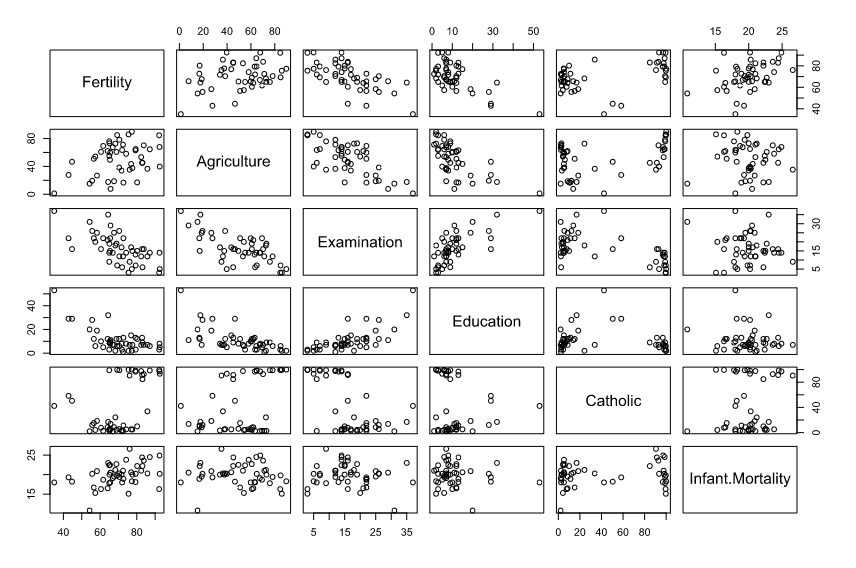
\includegraphics[width=0.8\linewidth]{Pairs}
\caption{Pairs Plot of Explanatory Variables}
\end{figure}

The Catholic variable is highly bimodal, with only a few points lying between the extremes of a majority Catholic or majority Protestant. Highly Catholic regions are typically less educated, score lower on the physical examinations, and are more agrarian. Given these extremes we decided to translate the Catholic variable into a categorical variable.\\
From the pairs plot we can also see that the examination parameter is not linear with fertility, this is a transformation we will consider if the variable has low significance.\\

\newpage
\section*{Fitting A Linear Model}

In order to determine possible data transformations, interactions, and variable selection, an initial linear fit of all explanatory variables is necessary. A multiple linear regression in RStudio yields the following output:

\begin{figure}[h!]
\centering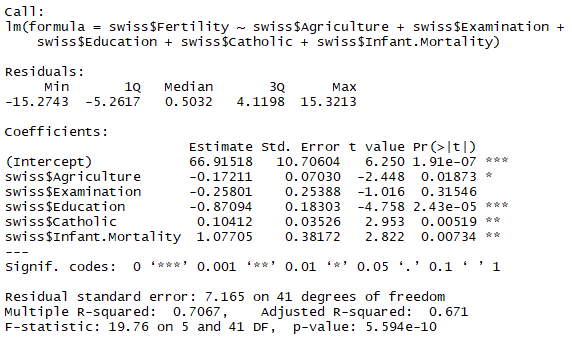
\includegraphics[width=0.8\linewidth]{SummaryBaseModel}
\caption{Summary Statistics for Base Model}
\end{figure}

We can see from our resulting fit that Examination does not immediately seem statistically significant - that is, we cannot confidently state that it's parameter value in a linear model is not zero. Given this low significance we decided to consider a transformation to the Examination variable. The plot suggests an inverse relationship between examination and fertility, as such we fit another linear model with \texttt{1/Examination}. 

\begin{figure}[h!]
\centering\includegraphics[width=0.8\linewidth]{ExamDenomModel}
\caption{Summary Statistics for Transformed Model}
\end{figure}









%% The Appendices part is started with the command \appendix;
%% appendix sections are then done as normal sections
%% \appendix

%% \section{}
%% \label{}

%% References
%%
%% Following citation commands can be used in the body text:
%% Usage of \cite is as follows:
%%   \cite{key}          ==>>  [#]
%%   \cite[chap. 2]{key} ==>>  [#, chap. 2]
%%   \citet{key}         ==>>  Author [#]

%% References with bibTeX database:

\bibliographystyle{model1-num-names}
\bibliography{sample.bib}

%% Authors are advised to submit their bibtex database files. They are
%% requested to list a bibtex style file in the manuscript if they do
%% not want to use model1-num-names.bst.

%% References without bibTeX database:

% \begin{thebibliography}{00}

%% \bibitem must have the following form:
%%   \bibitem{key}...
%%

% \bibitem{}

% \end{thebibliography}


\end{document}

%%
%% End of file `elsarticle-template-1-num.tex'.
